\pagebreak

\section{Inferenz Statistik}

\subsection{Motivation}

In der Schließenden Statistik werden die Ergebnisse (Parameter der Grundgesamtheit) überprüft und zu verifizieren, ob die usprüngelichen Annahmen über das Statisches Experiment zu treffen und ob die Stichprobe ausreichend Informationen enthält, eine solche Aussage zu treffen.
 
Die Essenz ist daher, anhand einer bekannten Stichproben $x$ einen unbekannten Parameter $\varTheta$ zu schätzen. Dafür konstruiert man einen \textit{Schätzer}.\\

Im Folgenden wird der Schwerpunkt der Beispiele darauf liegen, dass es sich bei den \textit{Parametern der Grundgesamtheit} um Parameter des \gls{SM} handelt - der Verteilungsfunktion. Bei den Regressionparameter gelten in den meisten Fällen die gleichen Definitionen. Die Definitionen beschreiben im Kern, wie mit den Daten der Stichproben umgegangen werden soll. Eine Einschränkung auf Parameter der Verteilungsfunktion ist in der Regel nicht gegeben.

\subsection{Schätztheorie}
\subsubsection{Statistik}
\paragraph{Definition Statistik und Abgrenzung zum Schätzer}
Eine \textit{Statistik} unterscheidet sich strukturell nicht von
\begin{itemize}
	\item von einer Schätzfunktion,
	\item einer Zufallsvariable (Abbildung),
	\item einem Punktschätzer oder
	\item einer messbaren Funktion (\refDefinition{Messbarkeitseigenschaft}).
\end{itemize}

\begin{Definition}{Statistik}
Sei $\left(\Omega,\SigmaAlgebra\right)$ ein \textit{messbarer Raum}\footnote{Hinweis zur Regression: Es wird hier nicht auf eine Wahrscheinlichkeitsraum verwiesen. Für die Abbildung werden nur die Werte aus $\Omega$ auf $\beta$ abgebildet. Für $\Omega$ kann auch gelten, dass es sich hierbei um einen Vektor handelt. So könnten verschiedenen Variablen $X$ und $Y$ auf einen andere Menge abgebildet werden.} und $\left(\beta, \SigmaAlgebraIndividuel{\beta}\right)$  ein weitere \textit{messbarer Raum}, so heißt eine \textit{messbare Abbildung}\footnote{Siehe Definition Messbare Abbildung \refDefinition{Messbarkeitseigenschaft}}
\begin{align}
	S: \left(\Omega, \SigmaAlgebra\right) \rightarrow \left(\beta, \SigmaAlgebraIndividuel{\beta}\right)
\end{align}
eine \textbf{Statistik}.
\end{Definition}

Im Kern steht, dass mit dieser Konstruktion Verteilungen und Bildmaße ermöglichen.\\
Der Unterschied, zwischen \textit{Statistik} und \textit{Schätzfunktion}, liegt in der Verwendung und Interpretation\footnote{Bei der Schätzfunktion werden nicht binden, weitere Eigenschaften gefordert. Somit bleibt die Definition die gleiche.}

\begin{description}
	\item[Statistik] Ziel ist es Ordnung und Struktur aus den vorhanden Informationen (Daten) zu gewinnen. Dabei soll die Beobachtungstiefe reduziert werden. 
	\item[Schätzfunktion] Ziel ist hier mit den vorhanden Daten ($\left(\Omega, \SigmaAlgebra \right)$) eine Auswertung zu gewinnen, um unbekannte Parameter/ Werte bestmöglich zu \textit{schätzen}. Die Schätzfunktion unterliegt hier Gütekriterien.
\end{description}

\paragraph{Beispiele für Statistiken und Schätzfunktionen}
Wie schon oben mehrmals erwähnt, eine Statistik teilt sich den Aufbau mit der Schätzfunktion und weiteren Objekten. Das Ziel ist jedoch eine Struktur oder eine Beschreibung (Deskriptive Statistik) zu bewinnen.\\

\begin{itemize}
	\item Die \textbf{Ordnungsstatistik} gibt den $i$-ten kleinsten Wert einer Stichprobe an.\\
	\item Eine \textbf{Teststatistik}, auch \textit{\textbf{Prüfgröße}} oder \textit{\textbf{Testgröße}} genannt, wird als Hilfsfunktion in der mathematischen Statistik im Bereich der Testtheorie verwendet. Bei einem Hypothesentest wird die \textit{Nullhypothese} abgelehnt, wenn die \textit{Teststatistik} einen gewissen Wert $k$ über oder unterschreitet.
\end{itemize}


Am Beispiel der Tesstatistik: Gegeben sei 
\begin{align}
	T: \Stichprobenmenge \rightarrow \R,
\end{align} die \textit{Teststatistik}, sowie ein \textit{statistischer Test}
\begin{align}
	\phi: \Stichprobenmenge \rightarrow [0,1],
\end{align}
mit 
\begin{align}
	\phi(X) = \begin{cases}
		1 & \text{falls} T(X) > k,\\
		0 & \text{falls} T(X) <= k
	\end{cases}
\end{align}

hierbei ist $k$ eine feste Zahl, die auch kriterischer Wert genannt. Ist $T$ ein $z-$Statistik, 
\begin{align}
	\overline{X} = \frac{1}{n}\left(X_1 + X_2 + \dots, X_n\right)
\end{align}
das Stichprobenmittel, $\Stichprobenmenge = \R^n$, ist eine typische Teststatistik
\begin{align}
	T(X) =\sqrt{n} \frac{\overline{X} - \mu}{\sigma}
\end{align}
Die \textbf{Teststatistik} ist standardnormalverteilt mit $T\sim \Normalverteilung{0,1}$. Für den $t-$Test ist die $t-$Statistik $t-$verteilt mit $T\sim t_{n-1}$.\\

Sei $X=\Menge{0,1}^n, \SigmaAlgebra = \Potenzmenge (X)$ und $\left(P_{\vartheta}\right)_{\vartheta \in \Theta} =\Menge{Ber(n, \vartheta)
| \vartheta \in \Theta}$ das \gls{SM}. Das \textit{Stichprobenmittel}, als Schätzfunktion für den Parameter $\vartheta$, ist gegeben durch das
\begin{align}
	\hat{\Theta}&: X \rightarrow [0,1]\Leerzeichen\text{mit}\Leerzeichen, \\
	&\hat{\Theta}(x) = \frac{1}{n}\sum_{i=1}^{n} x_i
\end{align}
\textit{Stichprobenmittel}. Eine Statistik könnte sein
\begin{align}
	M:X\rightarrow \R
\end{align}
mit $M(x)= \sum x_i$ als Statistik. Mit der Statistik $M$ wird nicht der Parameter $\vartheta = p$ geschätzt, sondern nur eine Informationsreduktion vorgenommen.\footnote{
	Quelle: \href{https://de.wikipedia.org/wiki/Statistik{\_}(Funktion)}{Statistik (Funktion)}, \href{https://de.wikipedia.org/wiki/Ordnungsstatistik}{Ordnungsstatistik}
}

\subsubsection{Schätzer}

Wie erwähnt, ein \textit{Schätzer} oder auch \textit{Schätzfunktion} oder \textit{Schätzstatistik} genannt, ist eine Funktion aus den Daten der Stichproben eine Aussage über unbekannte Parameter einer Grundgesamtheit zu tätigen.\\

\begin{Lemma-Definition}{Stichprobenraum}
% Stichprobenraum Geschwunges X \mathcal{X}
Ein \textit{Stichprobenraum} $\mathcal{X}_n$ besteht aus der Menge aller möglichen Stichprobenwerte $\left(x_1, \dots, x_n\right)\in X_n \subseteq \R^n$.
\end{Lemma-Definition}

\begin{Definition}{Schätzer/Schätzfunktion}
Sei $\Psi$ eine Statistik auf $\left(\Omega, \SigmaAlgebra\right)$ nach $\left(\beta, \SigmaAlgebraIndividuel{\beta}\right)$ (\refDefinition{Statistik}) und $X_1,\dots, X_n$ eine Stichprobe mit $(X_1,\dots,X_n)\in \Omega$. \\
Eine \textbf{Schätzer} für den Parameter $\vartheta$ oder den Funktionswert $\gamma$ ist eine Abbildung 
\begin{align}
	\Psi: \Omega \rightarrow \beta.
\end{align}
die messbar von $X_1,\dots,X_n$ abhängt.
\end{Definition}

Bei dem Schätzer\footnote{\href{https://de.wikipedia.org/wiki/Schätzfunktion}{Schätzfunktion}} sind drei Punkte besonders wichtig
\begin{itemize}
	\item Zu schätzen kann ein Wert $\vartheta$ oder eine Parameterfunktion/Kenngröße $\gamma$ sein.
	\item Ein Schätzer ist auch eine Zufallsvariable $\hat{\Theta}_n$ .
	\item Im Theoretischen wird mit den Zufallsvariablen $X_1,\dots,X_n$ im praktischen mit den Bildern der Zufallsvariablen/Stichprobenwerte $x_1,\dots,x_n$ gearbeitet.
\end{itemize}

\paragraph{Parameter oder Parameterfunktion}
In Verknüpfung mit der Entscheidungstheorie wird der Parameter nicht als Skalar abgebildet, sondern per Funktion, welche aus dem Parameterraum $\Theta$ in den Entscheidungsraum $\beta$ abbildet.
\begin{align}
	\gamma: \Theta \rightarrow \beta
\end{align}
Der Raum $\left(\beta, \SigmaAlgebraIndividuel{\beta}\right)$ wird auch \textit{Entscheidungsraum} genannt. \footnote{\href{https://de.wikipedia.org/wiki/Parameterfunktion{\_}(Statistik)}{Parameterfunktion}}.

Um genau zu sein, bildet die Entscheidungsfunktion in einen \textit{Entscheidungsraum} $(\beta, \SigmaAlgebraIndividuel{\beta}$.
\begin{Lemma-Definition}{Entscheidungsraum}
	Ein \textit{Entscheidungsraum} ist ein Messraum, bei dem die $\sigma-$Algebra alle einelementigen Mengen enthält, sodass $\forall \omega\in \Omega $ die Menge $\Menge{\omega} \in \SigmaAlgebraIndividuel{\beta}$ liegt. Beispielsweise ist $(\R, \SigmaAlgebraIndividuel{\R}$ ein Entscheidungsraum.
\end{Lemma-Definition}

\paragraph{Beispiel Parameterfunktion}
Für den Verteilungsparameter eine Bernoulli Verteilung $\vartheta$, wird dieser in der Regel mit dem Stichprobenmittel auf 
\begin{align}
	\gamma(\vartheta)=\vartheta
\end{align}
abgebildet.

Für die Normalverteilung wird für den Parameter $\sigma$ das Stichprobenmittel
auf 
\begin{align}
	\gamma(\sigma)=\sigma^2
\end{align}
abgebildet.

\paragraph{Symmetrie Schätzer als Zufallsvariable}

Wie in der Übersicht geschildert, wird aus der Schätzfunktion auch gleichzeitig eine eigene Zufallsvariable, siehe \ref{subsec_Dualitaet_DreiFaltigkeit}.

Die Abbildung $\Psi$ als Schätzer des Parameters $\vartheta$ ist gleichzeitig eine Zufallsvariable:

\begin{align}
	\hat{\Theta_n} := \Psi(X_1, \dots, X_n)
\end{align}
mit eigener Verteilung.

\begin{figure}[H]
	\centering
	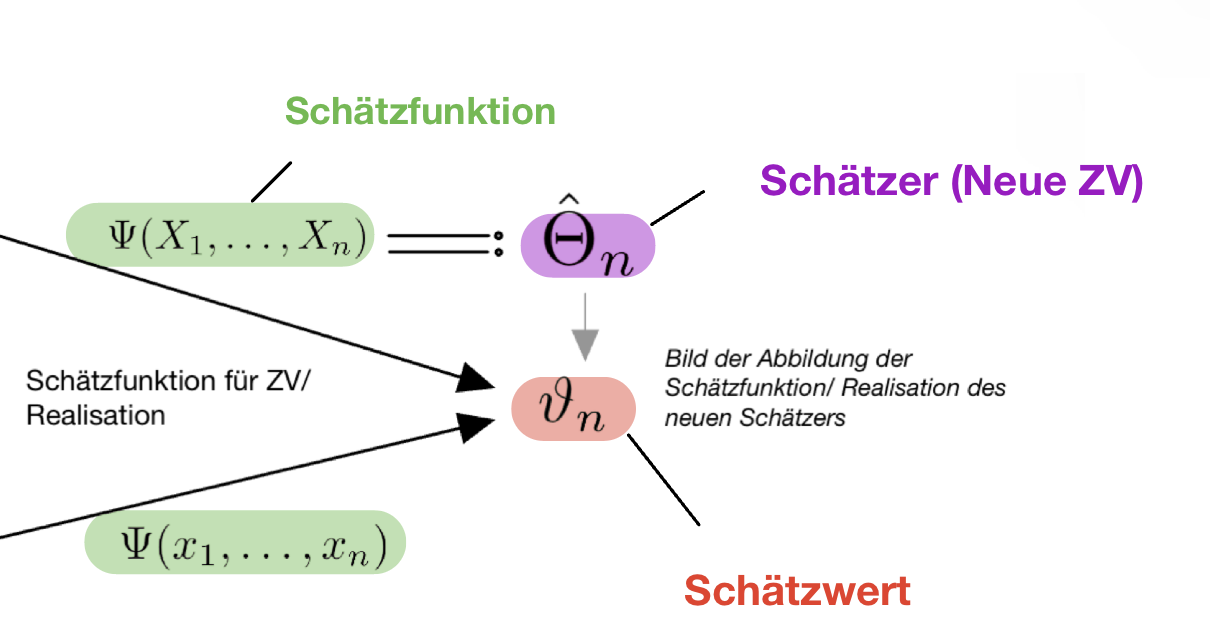
\includegraphics[width=0.7\linewidth]{attachment/chapter_13/Scc073}
	\caption{Drei Faltigkeit - Schätzer, Schätzfunktion und Schätzwert}
\end{figure}

Ebenso ist nochmals daraufhinzuweisen, dass es eine Unterschied zwischen der Funktion des Schätzers und des tatsächlichen Schätzwertes gibt.

\begin{figure}[H]
	\centering
	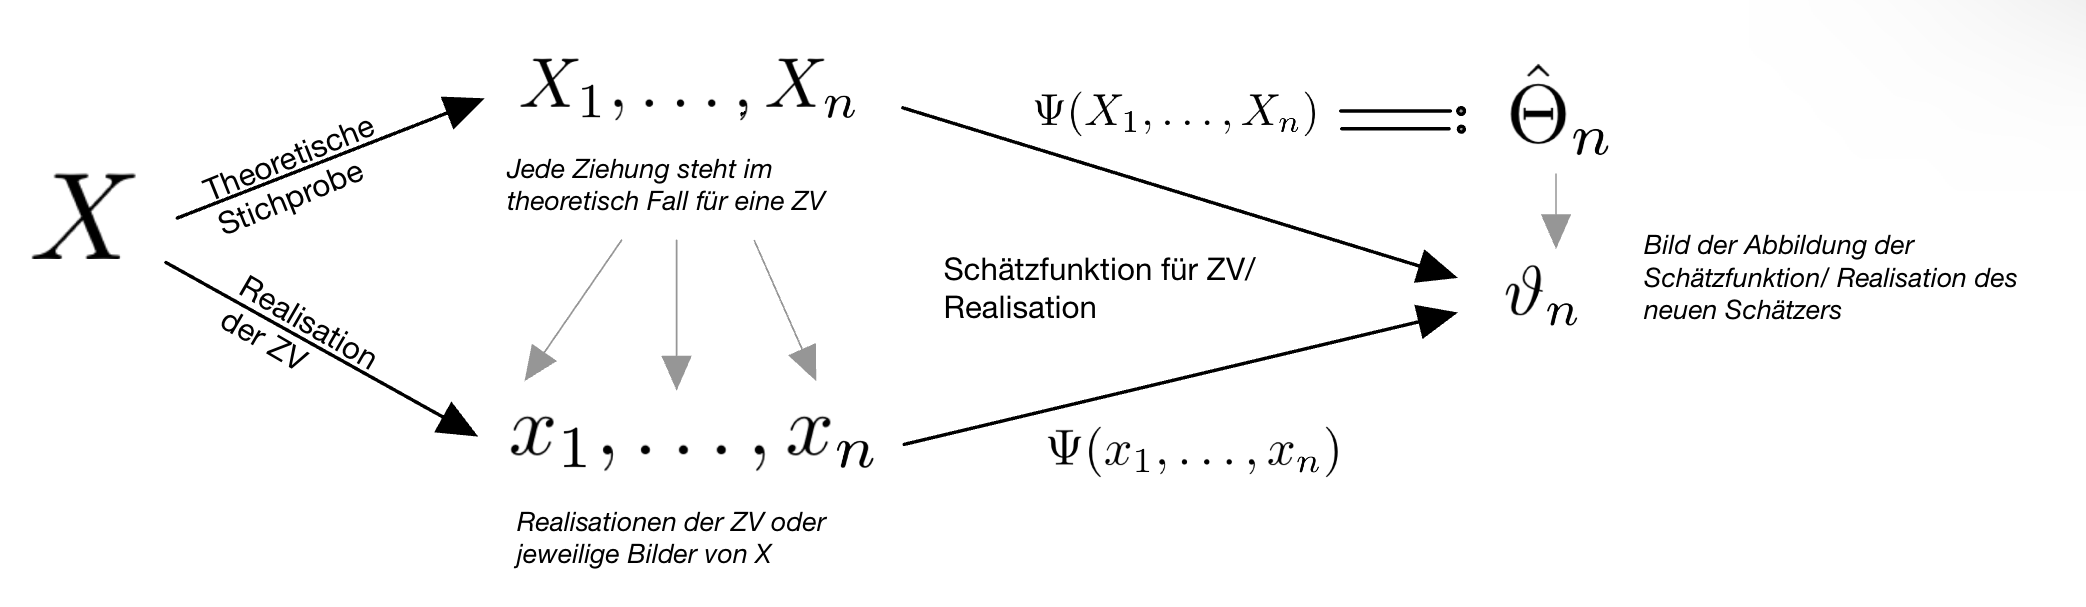
\includegraphics[width=0.7\linewidth]{attachment/chapter_13/Scc072}
	\caption{Theoretische und reale Betrachtung einer Stichprobe}
\end{figure}

Die Realisation von $\hat{\Theta}_n$ wird ebenfalls mit einem Dach versehen: $\hat{\vartheta}_n$

\paragraph{Verteilung der Schätzfunktion}
Wie im vorherigen Abschnitt erwähnt, ist die Schätzfunktion ebenso eine eigenen Zufallsvariaben $\hat{\Theta}$. Je nach Schätzfunktion besitzt diese eine eigene Verteilung. \\

Sei $X_1,\dots, X_n$ \gls{iid} Normalverteilt gilt für die Schätzfunktion, Stichprobenmittel
\begin{align}
	\hat{\Theta}\sim \Normalverteilung{\mu_X, \sigma_X/n}
\end{align}
Die Varianzschätzung $S_n^2$ um konstante Terme angepasst, verteilt sich wie folgt:
\begin{align}
	\frac{(n-1)S_n^2}{\sigma^2}\sim \mathbb{X}(n-1)
\end{align}
\footnote{
	Quelle: \href{https://de.wikipedia.org/wiki/SchätzfunktionVerteilungderSchätzfunktionen}{Schätzfunktion, Wiki}}
\subsubsection{Eigenschaften von Schätzern}
In der klassischen Inferenz Statistik sind
\begin{itemize}
	\item Erwartungstreue/ Mediantreue
	\item Effizienz
	\item Konsitenz,
	\item Suffizienz
	\item Normalität
	\item Linearität
	\item Robustheit
\end{itemize}
die wichtigsten Eigenschaften eines Schätzer $\hat{\Theta}_n$. Einige der Eigenschaften sind asymptotisch: Verhalten von $\hat{\Theta}_n$ für $n\rightarrow \infty$.

\paragraph{Erwartungs- und Mediantreue}
Für den Erwartungswert gilt wie unter \ref{paragraph: Erwartungswert}: 
\begin{align}
	\Erwartungswert{\hat{\Theta}_n} := \int \hat{\vartheta}d P_{\hat{\Theta}_n}(\hat{\vartheta}_n)
\end{align}
Wiederholter Hinweis: Diese Eigenschaft ist \underline{nur} wichtig, dass die Eigenschaft erfüllt ist!\\

\begin{Definition}{Erwartungstreue}
	Ein Schätzer $\hat{\Theta}_n$ heißt \textit{erwartungstreu} oder \textit{unverzerrt}, wenn 
	\begin{align}
		\Erwartungswert{\hat{\Theta}_n} = \gamma(\vartheta) \Leerzeichen \forall \vartheta \in \Theta.
	\end{align}
	oder simpler $\Erwartungswert{\hat{\Theta}_n} = \vartheta \Leerzeichen \forall$.
\end{Definition}

% Beispiel kommt aus dem Taschenbuch auf Seite 445
\textbf{Plausible Eigenschaft} Sei $\hat{\Theta}_n = \overline{X}_n = \frac{1}{n}\sum_i^nX_i$ das \textit{Stichprobenmittel} und $\vartheta = \Erwartungswert{X} = \mu$ mit $X_i \sim i.i.d.$ gilt
\begin{align}
	\Erwartungswert{\hat{\Theta}_n} &= 	\Erwartungswert{\overline{X}_n} \\
	&= 	\Erwartungswert{\frac{1}{n}\sum_i^nX_i} \\
	&= \frac{1}{n}\sum_i^n \Erwartungswert{X_i} \\
	&= \frac{1}{n}n \mu \Leerzeichen \text{mit}\Leerzeichen \Erwartungswert{X_i}=\mu_i = \mu \\
	&= \mu 
\end{align}
Der Schätzer $\overline{X}_n$ ist erwartungstreu. Wäre $\gamma(\mu)=\mu$, wäre der Schätzer ebenso erwartungstreu.

Bezüglich der Verteilung von $\overline{X}_n$ ist gegeben durch $X_i\sim \Normalverteilung{\mu, \sigma^2}$\footnote{Jede Zufallsvariable steht in dem Fall für das gleiche Merkmal. In Stichproben können jedoch auch mehrere Merkmale betrachtet werden.} $\overline{X}_n\sim\Normalverteilung{\mu, \sigma^2/n}$.\\

\textbf{Erwartungstreu, aber riskant} Sei der Schätzer
\begin{align}
	\Psi(X_1,\dots, X_n)\mapsto X_1,
\end{align}
so ist der Schätzer erwartungstreu für $\mu$. Dies ist jedoch ein unplausibler Schätzer, weil nur die erste Beobachtung berücksichtigt wird.\\

Abschluss: Es gibt viele \textit{erwartungstreue} Schätzer die unplausible sind. Ein \textit{idealer} Schätzer ist ein solcher welcher für $\forall \vartheta \in \Theta$ und $(x_1,\dots,x_n)$ den wahren Wert für $\gamma(\vartheta)$ schätzt.

\paragraph{Konsitenz}
Bei der \textit{Konsitenz} geht es darum, dass mit einer höhere Stichprobe, die Abweichung, zwischen den Schätzerwert und den Parameter gegen null geht.

\begin{Definition}{Erwartungstreue}
	Sei $\Psi(X_1,\dots, X_n)$ eine \textit{Schätzer} für die Funktion $\gamma(\vartheta)$ für alle $\vartheta\in \Theta$. Für den unbekannten Parameter $\vartheta$ der Grundgesamtheit heißt $\Psi$ für ein beliebiges $\epsilon >0$ \textit{\textbf{konsitenz}}, wenn
\begin{align}
	\lim_{n\rightarrow \infty} P_{\vartheta}\left(\lvert \Psi(X_1,\dots,X_n) - \gamma(\vartheta)\rvert>= \epsilon \right) = 0
\end{align}	  
\end{Definition}
Mit zunehmenden $n$ wird die Wahrscheinlichkeitsdichte des Parameters $\gamma(\vartheta)$ schmaler. Somit wird für jedes höhere $n$ mehr Fläche zwischen $\Psi \pm \epsilon$ liegen.
\begin{figure}[H]
	\centering
	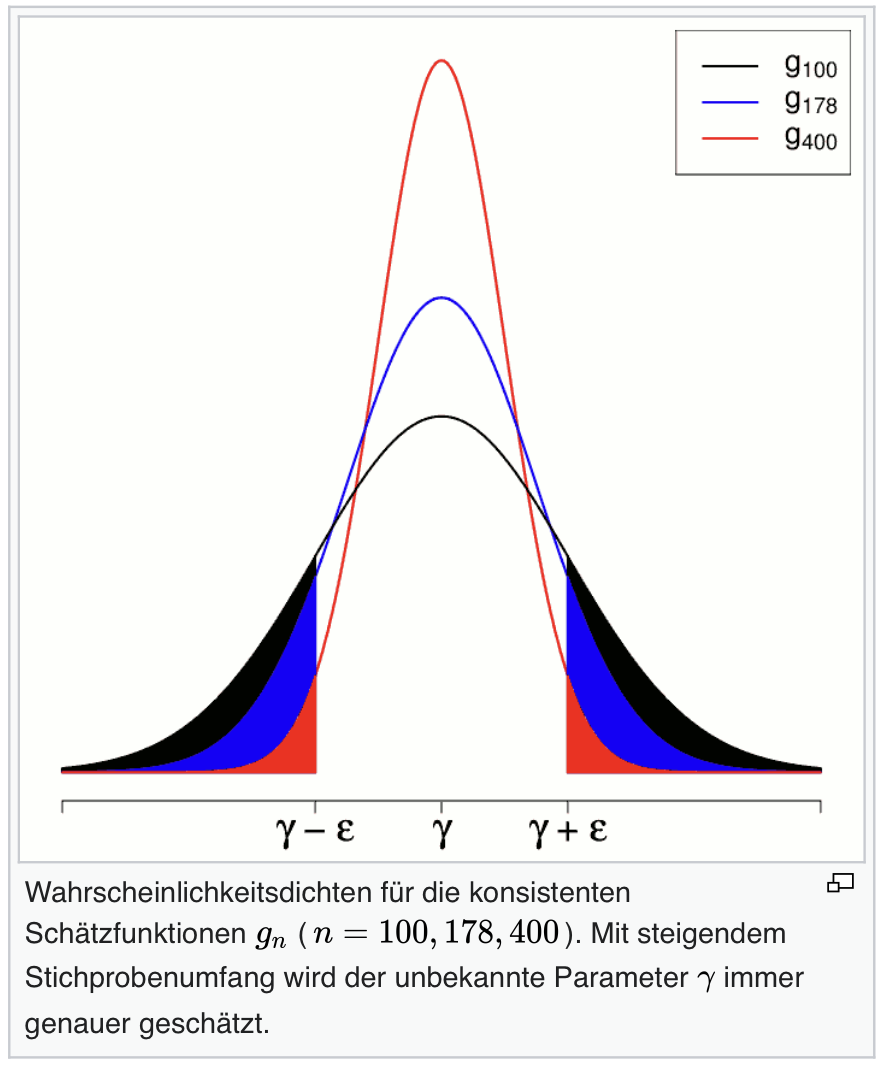
\includegraphics[width=0.5\linewidth]{attachment/chapter_13/Scc074}
	\caption{Wahrscheinlichkeitsdichte wird konzentierter um $\gamma$}
\end{figure}

\paragraph{Mittlere Quadratische Fehler (MSE)}
Die \gls{MSE} ist die Eigenschaft, welche untersucht, ob eine systematische Verzehrung vorliegt - ein Bias.

\begin{Definition}{Mittler Quadratischer Fehler (MSE)}
		Sei $\Psi(X_1,\dots, X_n)$ eine \textit{Schätzer} für die Funktion $\gamma(\vartheta)$ für alle $\vartheta\in \Theta$. Der \gls{MSE} definiert sich über 
\begin{align}
	MSE(\Psi, \gamma(\vartheta)):= \Erwartungswert{\lvert \Psi(X_1,\dots, X_n) -\gamma(\vartheta)\rvert^2} = \Varianz{\Psi} - Bias(\Psi)^2 , \vartheta\in \Theta  
\end{align}
\end{Definition}

Der Bias einer Zufallsvariablen definiert sich wie folgt:

\begin{Lemma-Definition}{Bias}
Sei $\Psi$ ein Schätzer für $\vartheta\in \Theta$:
	\begin{align}
		Bias(\Psi):= Bias(\Psi, \vartheta):= \Erwartungswert{\Psi} - \vartheta
	\end{align}
\end{Lemma-Definition}

\textbf{Herleitung des Mittleren Quadratischen Fehlers}\\

Durch gleichzeitige Addition und Subtration von $\Erwartungswert{\Psi}$ bleibt das Ergebnis unverändert:
\begin{align}
	MSE(\Psi) 
	&= \Erwartungswert{
		\left(
			\Psi(X_1,\dots, X_n) - \gamma(\vartheta)
		\right)^2
	} \\
	&= \Erwartungswert{
		\left(
			\Psi(X_1,\dots, X_n) 
			- \Erwartungswert{\Psi} + \Erwartungswert{\Psi} 
			- \gamma(\vartheta)
		\right)^2
	}  \Leerzeichen \\
&\text{mit}\Leerzeichen \Psi =  \Psi(X_1,\dots, X_n) \Leerzeichen \text{und}\Leerzeichen \gamma = \gamma(\vartheta)\\
	&= \Erwartungswert{
		\left(\Psi - \Erwartungswert{\Psi}\right)^2 
		+ 
		2\left(\Psi - \Erwartungswert{\Psi}\right)
		\left(\Erwartungswert{\Psi} - \vartheta \right) 
		- 
		\left(\Erwartungswert{\Psi} - \gamma \right)
	}\\
	&= \Erwartungswert{
		\left(\Psi - \Erwartungswert{\Psi}\right)^2 
		+ 
		2\left(\Psi - \Erwartungswert{\Psi}\right)
		\left(\Erwartungswert{\Psi} - \vartheta \right) 
		- 
		\left(\Erwartungswert{\Psi} - \gamma \right)^2
	}\\
\end{align}
Die Erwartungswert-Zerlegung erlaubt, dass der Erwartungswert auf die einzelnen additiven Teile angewandt werden kann.

\begin{align}
	\Erwartungswert{
		\left(\Psi - \Erwartungswert{\Psi}\right)^2
	}
	+
	\Erwartungswert{ 
		2\left(\Psi - \Erwartungswert{\Psi}\right)
		\left(\Erwartungswert{\Psi} - \vartheta \right) 
	}
	-
	\Erwartungswert{ 
		\left(\Erwartungswert{\Psi} - \gamma \right)^2
	}
\end{align}
Der Mittlere Termin mit $\Erwartungswert{\Psi} - \Erwartungswert{\Psi}$ wird zu Null. Der letzte Teil wir zu
\begin{align}
	\Erwartungswert{\left(\Erwartungswert{\Psi} - \gamma \right)^2} &=
	\Erwartungswert{
		\left(\Erwartungswert{\Psi} - \gamma \right)
		\left(\Erwartungswert{\Psi} - \gamma \right)
	}\\
	&= \left(\Erwartungswert{\Psi} - \gamma \right)^2\\
	&= Bias(\Psi)^2
\end{align}
Der erste Termin ist die Varianz, was zum Schluss ergibt:
\begin{align}
	MSE(\Psi) & = 	\Varianz{\Psi} - Bias(\Psi)^2
\end{align}
\footnote{Quellen hierfür sind: \href{https://wikis.hu-berlin.de/mmstat/MittlerequadratischeAbweichung(stochastisch)}{Uni Berlin}, \href{https://de.wikipedia.org/wiki/SchätzfunktionKonsistenz}{Schätzfunktion}}

\subsection{Methoden zur Schätzfunktionen Konstruktion}

In Folgenden werden Methode,
\begin{itemize}
	\item Momentummethode,
	\item Maximum-Likelihood Methode,
	\item Kleinstes Quadrate Methode,
	\item Bayer Methode
\end{itemize}
aufgezeigt, mit welche Schätzfunktionen konstruiert werden. Im Abschnitt zuerst wurde aufgezeigt, welche Eigenschaften eine Schätzer bewerten.\footnote{
\href{https://de.wikipedia.org/wiki/Schätzmethode(Statistik)}{Schaetzmethoden},
\href{https://www.uni-ulm.de/fileadmin/websiteuniulm/mawi.inst.110/lehre/ss13/Stochastik_I/Skript5.pdf}{Uni UlmStaMa}}

Die verschiedenen Verfahren liefern je nach Beispiel gleiche Ergebnisse, habe jedoch unterschiedliche Eigenschaften und Güte für ihre Ergebnisse. Somit konkurrieren die Methoden zum einen, zum anderen ergänzen sie sich.

\subsubsection{Momenten Methode}

Sei $x_i$ die Beobachtung von $n$ stochastisch unabhängig Zufallsvariablen $X_i$ mit bekanntem Verteilungstyp.\\
\paragraph{Herleitung}
Am Beispiel der Normalverteilung werde die Parameter $\mu$ und $\sigma$ theretisch durch 
\begin{align}
	m_1 = \Erwartungswert{X^1} = \mu \Leerzeichen \text{mit} \Leerzeichen m_2 = \Erwartungswert{X^2} = \sigma^2 + \mu^2
\end{align}
bestimmt.\footnote{Conjektor: Der 2-te theoretische Erwartungswert ist gleich des 1-ten und 2-ten zentralen Moments.}

Es gibt noch das \textit{empirische Moment} $\hat{m_k}$, welches sich aus den Realisation $x_i$ mit
\begin{align}
	\frac{1}{n}\sum_{i=1}{n}x_i^k 
\end{align}
bestimmt. Als Beispiel ist $\hat{m_k}$ der \textit{empirische Mittelwert}.

Die \textbf{simple Idee} ist, die \textit{theoretischen} mit dem \textit{empririschen Momenten} gleichzusetzen:
\begin{align}
	\hat{m_k} = m_k \Leerzeichen k = 1, \dots, n
\end{align}

Dabei benötigt es $p$ Gleichungen, um $p$ Parametern zu finden.\\

\textbf{Beispiel} Um die Parameter der Normalverteilung $\mu$ und $\sigma^2$ zu schätzen, wird
\begin{align}
	m_1(\mu, \sigma^2) &= \Erwartungswert{X_i} = \frac{x_1 + \dots, x_n}{n}\Leerzeichen \text{und}\\
	m_2(\mu, \sigma^2) &= \Erwartungswert{X_i^2} = \frac{x_1^2 + \dots, x_n^2}{n}
\end{align} gleichgesetzt. Sei $m_1(\mu, \sigma^2) = \overline{x}$. Es wird erhalten
\begin{align}
	\hat{\sigma^2} = \frac{1}{n}\sum (x_ - \overline{x})^2.
\end{align}
\paragraph{Konzept}

\begin{description}
	\item[Vorteil] Die Vorteil dieser Methode liegen in der einfachen Berechnung, selbst wenn das Gleichungssystem durch nicht-lineare Gleichungen bestimmt wird und die Lösung iterativ gefunden werden muss. Die Momentenmethoden kann auch bei abhängigen Zufallsvariablen eingesetzt werden. Während die \gls{MLE} eine komplizierte Lösung benötigt. 
	\item[Nachteil] Die Einfachkeit der Berechnung ist auch gleichzeitig der Nachteil. Nicht alle Informationen aus einer Stichprobe werden genutzt. So kann bei kleinen Stichproben der Schätzwert außerhalb des Parameterraums liegen. Ebenso sind Schätzer meist nicht effizient. So zum Beispiel ist bei einer Gleichverteilung Momentenschätzer weniger effizient als \gls{MLE}.
\end{description}


\subsubsection{Maximum Likelihood Schätzer}

Sei $x_i$ die Beobachtung von $n$ stochastisch unabhängig Zufallsvariablen $X_i$ mit bekanntem Verteilungstyp.\\

Die \gls{MLE} wurde von Carl Friedrich Gauß entwickelt. Bei der \gls{MLE} wird der Schätzwert für den unbekannten Parameter $\vartheta$ bestimmt. Dieser Schätzer bestimmt sich, dass gefragt, wird, welcher Parameter weißt die höchste Wahrscheinlichkeit auf, dass die Stichprobe $x=(x_1,\dots, x_n)$ vorkommt.\footnote{Im Regelfall werden die Parameter der Verteilung gesucht.}

\begin{description}
	\item[Vorteile] Der Vorteil der \gls{MLE} liegt in den Eigenschaft von Schätzern der \gls{MLE}: 
\begin{itemize}
	\item effizient und
	\item asymthotische Effizienz, ebenso können vergleichsweise einfach
	\item verschiedenen Signifikanztests durchführen.
\end{itemize}
	\item[Nachteile] Ein großer Nachteil ist, dass der Verteilungstype für $X_i$ vorher bekannt sein muss. Ist diese Wahl falsch, so kommt es zu Verzerrungen in den Ergebnissen. Wenn die Parameter durch numerische Maximierung gefunden werden müssen, besteht das Risiko, dass es sich um ein lokales nicht ein globales Maximum handelt.
	\item[Vergleich] Ist $X_i$ normalverteilt, liefert \gls{MLE} und die Momentenmethode das gleiche Ergebnis für die Parameter. Der Unterschied liegt im systematischen Fehler.	Bei der Momentenmethode kommt es zu einem kleineren Fehler in der Standardabweichung.
\end{description}

\paragraph{Herleitung}
Für \gls{MLE} wird entweder angenommen, dass die Verteilung diskret oder absolute stetig ist.\\

Gegeben eine Familie diskreter Familie von Verteilungen $P^X = \Menge{P^X_\vartheta, \vartheta\in\Theta}$, soll auf Grundlager der Beobachtungen von $X$ der Parameter $\vartheta$ geschätzt werden. 

\begin{Definition}{Maximum-Likelihood Funktion}
	Die Funktion
	\begin{align}
	 \MaximumLikelihoodFunktion \stackrel{def}{=} P^X_\vartheta(x) = P_\vartheta(\Menge{X=x})
	\end{align}
	heißt \textit{Maximum-Likelihood Funktion}. Die \MaximumLikelihoodFunktion wird als Funktion abhängig nur vom Parameter $\vartheta$ verstanden, weshalb es ausreicht, wenn $\mathbb{L}(\vartheta)$ geschrieben wird.
\end{Definition}
\begin{itemize}
	\item Bei einem fixen $\vartheta$ ist die \gls{MLF} gleich der Zähldichte von $X$.
	\item Die Funktion 
	\begin{align}
		\MaximumLikelihoodFunktion = \mathbb{L}\left(x_1,\dots,x_n;\vartheta \right) = P^X_\vartheta\left(X_1=x_1, \dots, X_n=x_n\right)
	\end{align}
	gibt an, mit welcher Wahrscheinlichkeit die Kombination (Stichprobe) gegeben des unbekannten Parameters $\vartheta$ ist.
	\item Wenn die Ziehungen $X_i$ unabhängig und identisch ist, gilt
	\begin{align}
		\MaximumLikelihoodFunktion =  P^X_\vartheta(X_1=x_1)\cdot P^X_\vartheta(X_n=x_n) = \prod P^X_\vartheta(X_i=x_i)
	\end{align}
\end{itemize}

Das Grundprinzip ist
\begin{align}
	\MaximumLikelihoodFunktion \rightarrow \max.
\end{align}
Der Maximum-Likelihood Schätzer ist definiert durch
\begin{align}
	\Psi_{ML} = \arg\max_{\vartheta\in \Theta} \MaximumLikelihoodFunktion.
\end{align}
Es kann sein, dass es mehrer Lösungen gibt.


\subsubsection{Methode der Kleinsten Quadrate}
\paragraph{Allgemeine Anwendung}
Die \gls{MKQ} kann in allgemeiner Form und angepasst für die Regression definiert werden. Der erste Fall ist der wenig verwendete Fall. Der Schwerpunkt dieser Methode liegt darin, Schätzer für die Parameter des \gls{GML} zu bestimmen.\\

Im Allgemeinen Fall\footnote{Mathematik, Arens, Seite 1533} wird ein Parameter $\hat{\mu}$ bestimmt, welcher einen Abstand zwischen den Werten der gesuchten Stichproben $y$ und und einer festgelegten Grenze $m$ minimiert. Für $m$ können verschiedenen Werte vorliegen. Meist handelt es sich um den zu bestimmenden Erwartungswert. Im Fall einer Regression handelt es sich um den Vektor, der vom \gls{GML} produziert wird und gespeißt durch mit erhaltenen Werte $x$. Dieser soll nach den erzeugten Stichprobenwerten $y$ kommen. Dabei ist die Gleichung abhängig von den \textit{\textbf{variablen}} Parametern $\beta$. Im Regressionsfall ist es jedoch auch der Erwartungswert $\Erwartungswert{Y}$ des \gls{GML}.

\begin{Definition}{Kleinste-Quadrat Methode}
	Die \gls{MKQ} schätzt den Wert für den unbekannten Wert $\mu$ durch $\hat{\mu}\in\Theta$, den \textit{Vektor der minimalsten Abstände zu} $y$:
	\begin{align}
		\hat{\mu} = \arg\min_{m\in\Theta} ||y - m||^2.
	\end{align}
	Es gilt $||y - \hat{\mu}||^2 \leq ||y - m||^2$ für alle $m\in \Theta$.
\end{Definition}
Dies bedeutet, gegeben der Stichproben $y$ der Zufallsvariable $Y$ wird ein Vektor $m$ gesucht, welcher den Abstand zwischen $\hat{\mu}$ und $y$ minimal ist. \footnote{Die Operator $\arg\min$ gibt nicht den Funktionswert wie $\min$ zurück, sondern die Menge der gesuchten Parameter. In dem Fall $m$.}\\ 

\paragraph{Anwendung bei der Regression}

In Fall eines \gls{GML} ist $m$ durch den Erwartungswert des Regressionsmodell in Abhängigkeit des Parameter $\beta$ gegeben. Gleichfalls wird in das Modell die Ausprägungen der abhängigen Variable $X$ eingesetzt. Zu vergleichen sind ist die Stichprobe $y$:
\begin{align}
	\hat{\beta} &= \arg\min_{\beta\in\Theta} ||y - \Erwartungswert{y} ||^2\\
	 &= \arg\min_{\beta\in\Theta} ||y - \Erwartungswert{\beta x} ||^2\\
\end{align}


Hier hängt der Erwartungswert $\Erwartungswert{Y}$ direkt oder durch eine bekannte Funktion von den Parametern (den zu schätzenden Parametern) sowie einer Störgröße ab. Daher bestimmt man die gesuchten Parameter so, dass die Summer der Störgrößen möglichst klein sind.\\

Das einfache Beispiel ist die lineare Regression $Y=\beta_0 + \beta_1X$, mit den Parametern $\beta_0$ und $\beta_1$.\footnote{Je nach Modell, wird hier schon von einer Zufallsvariablen $Y$ oder nur einer Variablen $Y$ gesprochen. In dem Beispiel wird der zweite Fall betrachtet.} Diese wird von einer Störgröße, einer Zufallsvariablen $\epsilon_i$ überlagert, somit beobachtet man nur $(y_i,x_i)$ mit $Y_i = \beta_0 + \beta_1X_i + \epsilon_i $. Für die Zufallsvariable $Y_i$ gilt
\begin{align}
	\Erwartungswert{Y_i} = \beta_0 + \beta_1X_i,
\end{align}
wobei $\Erwartungswert{\epsilon_i} = 0$ ist. Die Funktion der Summe der quadrierten Störgrößen 
\begin{align}
	\sum \left(y_i - (\beta_0 + \beta_1x_i)	\right)^2 \rightarrow \min
\end{align}
um die Schätzwerte für $\beta_0$ und $\beta_1$ zu finden.

Für ein lineares Modell gilt,	 sind die Schätzer für $\beta_0, \beta_1$ gegeben durch die Minimierung der Summer der Quadrate
\begin{align}
	(\Psi_{KQ, \beta_0}, \Psi_{KQ,\beta_1}) := \arg\min \sum (Y_i - \beta_0 - \beta_1X_i)^2.
\end{align}

Versteht man die Schätzfunktion $\Psi_{KQ}$ als Funktion von $\beta_0$ und $\beta_1$, und wie im Beispiel unten, wird diese minimiert, erhält man für $\beta_0$ die Lösung
\begin{align}
	\beta_1 = \frac{Cov_{X,Y}}{Var_{X}}
\end{align}
und $\beta_0$ wird durch einsetzen gefunden.
	
\begin{description}
	\item[Vorteil] Es benötigt eine Annahmen über die Verteilung von $Y_i$. Es wird nur der Zusammenhang zwischen dem Erwartungswert $\Erwartungswert{Y_i}$ und den Parametern benötigt. Die Methode ist daher für ein breites Spektrum anzuwenden. Die große Anwendung findet die Methoden, wenn nicht eine einzelne Variablen im Fokus steht, sondern der Zusammenhang verschiedener Variablen.
	\item[Nachteil] Der Vorteil ist auch gleichzeitig der Nachteil. Weil Informationen über die Verteilung von $Y_i$ nicht genutzt werden, weißen die Schätzer schlechtere Eigenschaften als Funktionen der \gls{MLE} auf. Weißt die Regressionsfunktion einen nicht linearen Zusammenhang auf, müssen die Parameter numerisch geschätzt werden.
\end{description}

\paragraph{Schätzeigenschaften}

Bei der Schätzfunktion und den Eigenschaften muss unterschieden werden, zwischen den Lösungen von $\Psi_{KQ,\beta_1}$ und $\Psi_{KQ,\beta_1}$ selbst.

Die \textit{erwartungstreue} für $\beta_1$ ergibt sich, wenn
\begin{align}
	\Erwartungswert{\hat{\beta_1}} &= \Erwartungswert{\frac{Cov(X,Y}{\Varianz{X}}}\\
	&=\beta_1 + \Erwartungswert{\frac{Cov(X,\epsilon}{\Varianz{X}}},
\end{align}
und somit der Erwartungswert $Cov(X,\epsilon)=0$ ist, und somit der Schätzer für $\beta_1$ \textit{erwartungstreu}.

\begin{figure}[H]
	\centering
	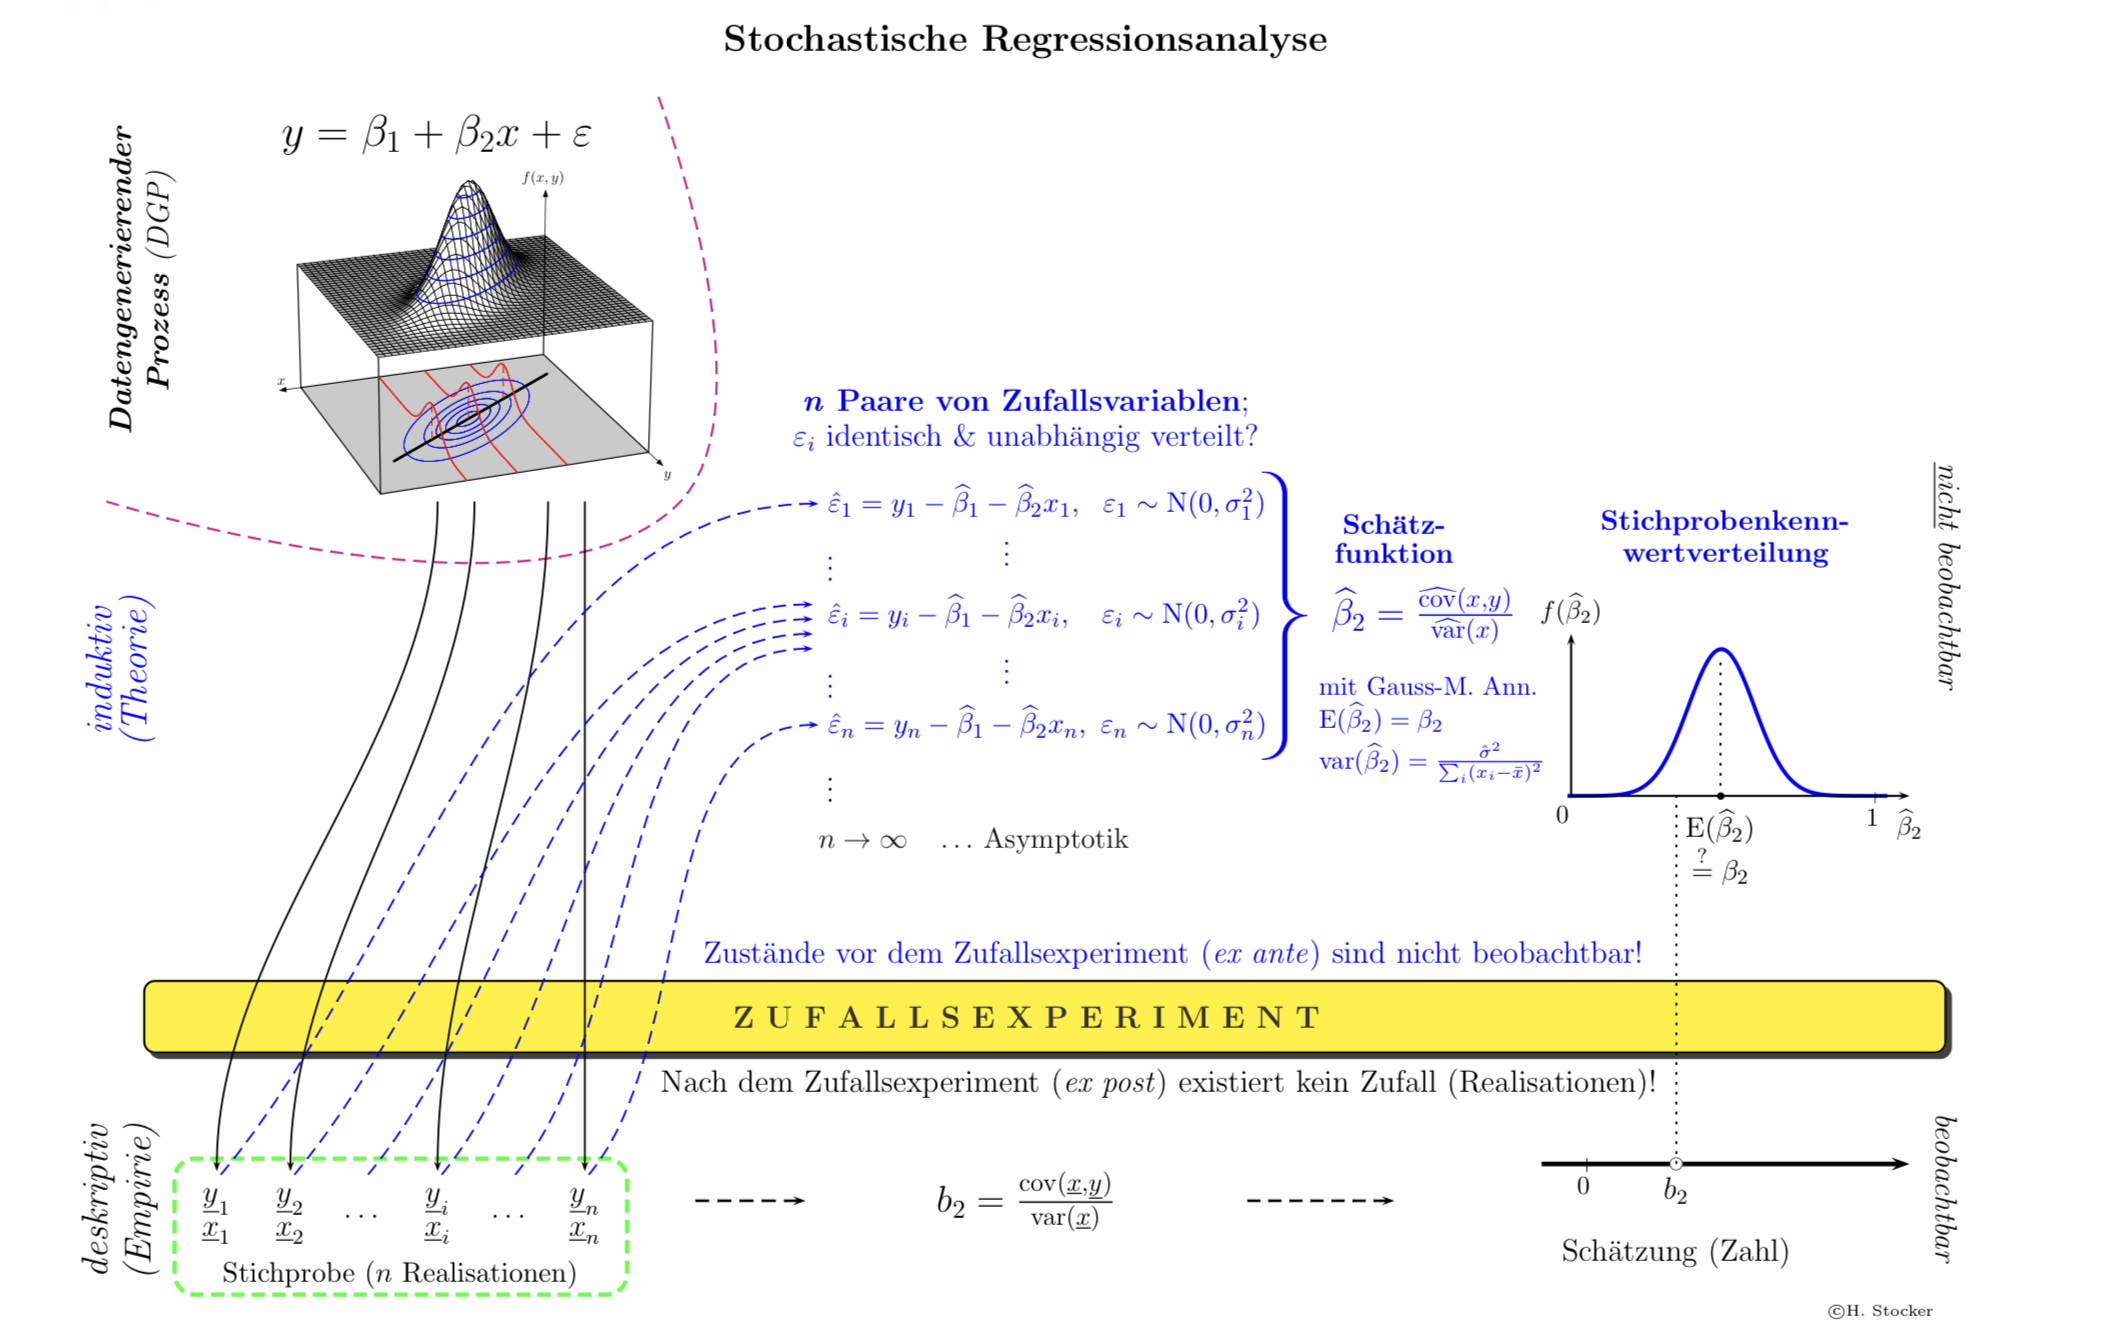
\includegraphics[scale = 0.1]{attachment/chapter_13/Scc076} % Screenshot konnte nicht gespeichert werden. Am 24.06.22 wurde das Foto in der Bibliothek gespeichert.
\end{figure}


\subsubsection{Anwendung an einem Beispiel}
In einem Spiel kann man 1 Euro mit der Wahrscheinlichkeit $p$ verlieren, $1-2p$ gewinnen und $p$ weder gewinnen noch verlieren.\\
Das Spiel wird sechs mal gespiel mit der Ziehung
\begin{align}
	x = (-1,1,-1,0,1,1).
\end{align}
Wie groß ist der Wert für $p$?\\

\paragraph{Maximum-Likelihood Methode (MLE)}
Mit der \gls{MLE} wir der Erwartungswert für $p$ wie folgt berechnet.
\begin{align}
	&\arg\max_{p} P(X_1=-1, X_2=1, X_3=-1,X_4=0, X_5=1, X_6=1)\\
	 &= P(X_1=-1)\cdot P(X_2=1) \cdot P(X_3=-1)\cdot P(X_4=0) \cdot P(X_5=1)\cdot P(X_6=1)\\ 
	 &= (1-2p)^3p^3 \\
	 &\rightarrow p=0,25\\
\end{align}
Lösung:

\begin{figure}[H]
	\centering
	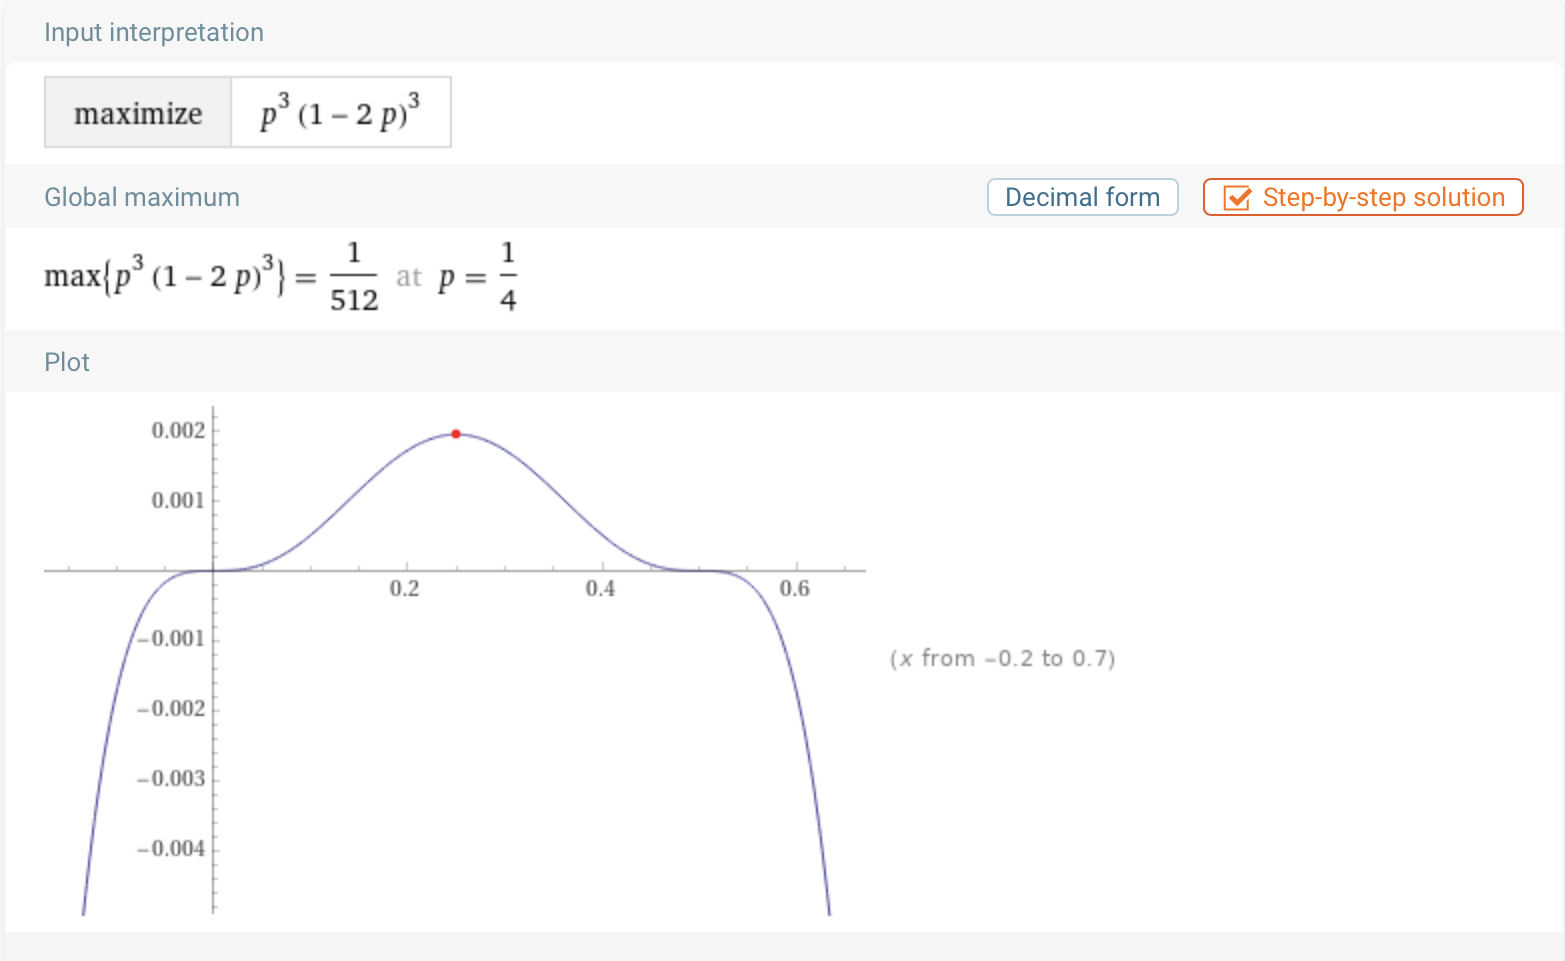
\includegraphics[scale = 0.3]{attachment/chapter_13/Scc075}
\end{figure}

\paragraph{Methode der Kleinsten Quadrate}
Der interessante Teil ist, dass für den \gls{KQS} der Erwartunswert $\Erwartungswert{X_i}$ benötigt wird, siehe Methode oben. Dieser wird als \textit{nicht geschätzer} Erwartungswert betrachtet. Jede Ausprägung wird betrachtet und mit der zugeordneten Wahrscheinlichkeit betrachtet:\footnote{Achtung: Es für für $\Erwartungswert{X_i}$ nicht ein separater Schätzer eingesetzt, $\Erwartungswert{X_i} = -p + p - p + 0 + p + p$ ist falsch.}
\begin{align}
	\Erwartungswert{X_i} &= (1)\cdot (1-2p) + (0)\cdot (p) + (-1)\cdot p \\
	&=1-2p - p\\
	&=1-3p
\end{align}
Für jede Ziehung wird jetzt die quadratische Differenz zwischen der tatsächlichen Ausprägung und der erwarteten Ausprägung bestimmt.
\begin{align}
	\Psi_{KQ,p} &= \arg\min_{p\in [0,1]}  (-1 - \cdot \Erwartungswert{X})^2 + (1 - \cdot \Erwartungswert{X})^2 \\
	 &+ (-1 - \cdot \Erwartungswert{X})^2 + (0 - \cdot \Erwartungswert{X})^2 + (1 - \cdot \Erwartungswert{X})^2 + (1 - \cdot \Erwartungswert{X})^2\\
	&= \arg\min_{p\in [0,1]}  (-1-(1-3p))^2 + (1 -(1-3p))^2 + (-1 -(1-3p))^2 \\ & + (0 -(1-3p))^2 + (1 -(1-3p))^2 + (1 -(1-3p))^2\\ 
	&= \arg\min_{p\in [0,1]}  9 - 30p +54p^2
\end{align}
In im Konzept der Methode besprochen, wird nicht der Funktionswert gesucht, sondern die $p$, welche die Funktion $9-30p+54p^2$ minimiert. Mit der pq-Formel erhält man $\Psi_{KQ,p} = p_{KQ} = 5/18$.

Wie man sieht, unterscheidet sich bei diesem Beispiel, der Wert für den Schätzer von $p$ abhängig von der Methode.